\documentclass[tikz,border=8pt]{standalone}
% Shared look for every TikZ diagram. Load with \input{../../tools/tikz-style.tex}
\usepackage[T1]{fontenc}
\usepackage{lmodern}
\renewcommand{\sfdefault}{lmr}  % diagrams use the same serif as the text
\usetikzlibrary{arrows.meta, positioning, shapes.geometric, calc, fit, backgrounds}
\definecolor{cblue}{HTML}{4C78A8}
\definecolor{corange}{HTML}{F58518}
\definecolor{cgreen}{HTML}{54A24B}
\definecolor{cred}{HTML}{E45756}
\definecolor{cpurple}{HTML}{B279A2}
\definecolor{cgrey}{HTML}{6B6B6B}
\tikzset{
  every picture/.style={font=\sffamily, line width=1.2pt},
  box/.style={draw=#1, fill=#1!12, rounded corners=4pt, align=center, inner sep=7pt, minimum height=1.1cm},
  box/.default=cgrey,
  arrow/.style={-{Stealth[length=3mm]}, draw=cgrey, line width=1.4pt},
  title/.style={font=\sffamily\bfseries\Large},
  note/.style={font=\sffamily\small, text=cgrey, align=center},
}
\AtBeginDocument{\hyphenpenalty=10000 \exhyphenpenalty=10000}

\begin{document}
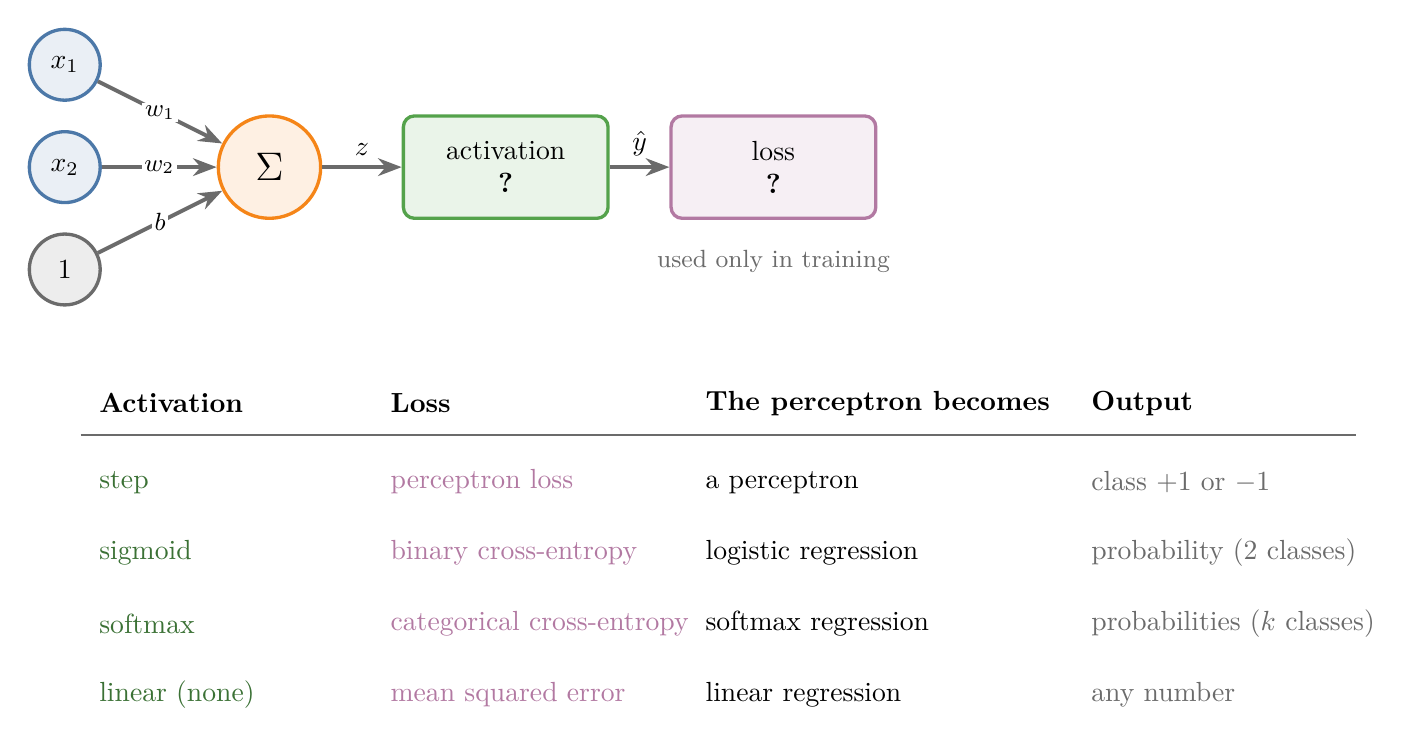
\begin{tikzpicture}
  \tikzset{inp/.style={circle, draw=cblue, fill=cblue!12, minimum size=0.9cm}}
  \node[inp] (a) at (0,1.3) {$x_1$};
  \node[inp] (b) at (0,0) {$x_2$};
  \node[inp, draw=cgrey, fill=cgrey!12] (c) at (0,-1.3) {$1$};
  \node[circle, draw=corange, fill=corange!12, minimum size=1.3cm, font=\Large] (s) at (2.6,0) {$\Sigma$};
  \foreach \n/\l in {a/w_1, b/w_2, c/b} \draw[arrow] (\n) -- node[fill=white, inner sep=1pt, font=\small] {$\l$} (s);
  \node[box=cgreen, minimum width=2.6cm, minimum height=1.3cm] (act) at (5.6,0) {activation\\\textbf{?}};
  \node[box=cpurple, minimum width=2.6cm, minimum height=1.3cm] (loss) at (9.0,0) {loss\\\textbf{?}};
  \draw[arrow] (s) -- node[above] {$z$} (act);
  \draw[arrow] (act) -- node[above] {$\hat{y}$} (loss);
  \node[note, below=0.25cm of loss] {used only in training};
  % table
  \begin{scope}[yshift=-3.0cm]
  \foreach \x/\h in {0.3/Activation, 4.0/Loss, 8.0/The perceptron becomes, 12.9/Output}
    \node[anchor=west, font=\sffamily\bfseries] at (\x,0) {\h};
  \draw[cgrey, line width=0.8pt] (0.2,-0.4) -- (16.4,-0.4);
  \foreach \y/\act/\lss/\what/\out [count=\i] in {
      -1.0/step/perceptron loss/a perceptron/class $+1$ or $-1$,
      -1.9/sigmoid/binary cross-entropy/logistic regression/probability (2 classes),
      -2.8/softmax/categorical cross-entropy/softmax regression/probabilities ($k$ classes),
      -3.7/linear (none)/mean squared error/linear regression/any number}
  {
    \node[anchor=west, text=cgreen!70!black] at (0.3,\y) {\act};
    \node[anchor=west, text=cpurple] at (4.0,\y) {\lss};
    \node[anchor=west] at (8.0,\y) {\what};
    \node[anchor=west, text=cgrey] at (12.9,\y) {\out};
  }
  \end{scope}
\end{tikzpicture}
\end{document}
